\section{MOTION DETECTION EXPERIMENTATION}
The rotational and translational SD motion detection experiments were designed identically such that the resulting SD dataset would be in a standard format. The following experimental parameters were the same for both experiments: experimental stimulus conditions, number of randomized trials per experiment, timeline of experimental events per trial, experimental protocol, and motion simulation system. In order to validate our SD dataset using our motion simulator platform, we followed recent motion detection protocols that also used motion simulator platforms such as the Moog 6-degree-of-freedom (DOF) motion platform \cite{BermudezRey_2016_Vestibular}, \cite{Hartmann_2014_Direction}, \cite{Karmali_2017_Multivariate}, \cite{Valko_2012_Vestibular}. Recent motion simulator-based motion detection protocols report motion detection thresholds in terms of speed, thus manipulating speed as an experimental condition instead of acceleration. Robotic motion planning is easier and more accurate for speed control than acceleration control. Finally, to create a diverse dataset of vestibular and proprioceptive SD responses, perceptual responses were measured using a 3 x 3 block design testing a randomized combination of angular or linear axis motion, axial direction, and speed. A total of 32 participants, for both experiments, received the same experimental instructions and protocol while using the motion simulator.

\subsection{EXPERIMENTAL DESIGN}
\label{EXPERIMENTAL_DESIGN}
% 1st paragraph
The axis experimental condition had three parameters, cabin movements for rotation were roll (RO), pitch (PI), and yaw (YA), and translation included left/right (LR), forward/backward (FB), and up/down (UD). In addition, minuscule sinusoidal vibrational noise of, 1-2 cm in amplitude and frequency greater than 10Hz was added to the non-stimulated axes to mask the sound of the motor for the selected stimulus. Because vibrational noise was present, the participants were exposed to a more realistic aviation environment. Furthermore, the additional vibration helped reduce movement detection thresholds, such that the task was realistically challenging \cite{Chaudhuri_2013_Wholebody}. The axial direction experimental condition had two parameters: positive or negative direction. Figure \ref{fig1} A depicts both the axis and axial direction conventions for both the rotational and translational experiments; the grey Cartesian coordinate frame represents the simulator cabin. The cabin could move in both rotation (RO, PI, YA) and translation (LR, FB, UD) via the input stimulus and/or participant control. The black outlined squares and circles in Figure~\ref{fig1}A denote positive directional movement (RollP, PitchP, YawP, Right, Forward, Down), where squares and circles correspond to rotational and translation movement respectively. Non-outlined squares and circles indicate negative directional movement (RollN, PitchN, YawN, Left, Backward, Up). Figure~\ref{fig1}B shows the mapping of participants’ joystick movements to the cabin movement.

% -------------------- Figure 1 --------------------
\begin{figure}[htp]
\begin{center}

\includegraphics[width=1.0\linewidth]{figures/figure1.eps}
\end{center}
\caption{Axial and directional motion convention for cabin (A) and joystick (B).}
\label{fig1}
\end{figure}
% --------------------

\noindent The speed experimental condition had two parameters; a slow near below-threshold (sub) speed where motion was difficult to detect and a fast above-threshold (sup) speed where motion detection was easier to detect. Some talented participants could detect sub speed movement, therefore this lower limit perceptual stimulation was emphasized to be at ``near below-threshold" instead of at a below-threshold speed. In the motion detection literature, our speed parameters are known as motion detection thresholds measured in terms of Hz, which is a frequency measure of deg/s or cm/s depending on whether the stimulus motion is in rotation or translation respectively. Rotational and translational, sub and sup speed selection was based on reported experimental design thresholds from motion detection literature that accommodated the motion constraints of the simulation system \cite{Hartmann_2014_Direction}, \cite{BermudezRey_2016_Vestibular}, \cite{Karmali_2017_Multivariate}, \cite{Valko_2012_Vestibular}, \cite{Melvill_1978_Vertical}. The Rotational and translation task sub \& sup speeds were 0.5 Hz (deg/s) \& 1.25 Hz (deg/s) and 3.75 Hz (cm/s) \& 15 Hz (cm/s) respectively; implying that acceleration was constant at 0.5 deg/$\textrm{s}^{2}$ \& 1.25 deg/$\textrm{s}^{2}$ and 3.75 cm/$\textrm{s}^{2}$ \& 15 cm/$\textrm{s}^{2}$ respectively.

\indent Figure \ref{fig2}A and \ref{fig2}B show a typical position trajectory when the participant did not respond and when the participant responded during phase A respectively, demonstrating that the experimental phases and trial length were dependent upon the participant’s initial response. A single trial was composed of four different phases, as denoted by the timeline in Figure \ref{fig2}, in which participants were tasked to give feedback to specific visual and vestibular stimuli per phase. During phases a and b, participants could move the simulator using the joystick in any of the rotational or translational axes to counteract the perturbation. Joystick control was in terms of velocity control because it allowed for fast and smooth responses. Timeline A occurred when the participant did not respond in phase A, it consisted of three phases: (a Detection) motion stimulation of the cabin using a smoothed ramp forcing function, (c Reinitialization) cabin reinitialization to the initial orientation or position, (d Rest) cabin and participant at rest. Timeline B occurred when the participant responded in phase a, the four phases consisted of: a Detection, (b Active control) participant active control, c Reinitialization, d Rest. For both timeline A and B, visual and vestibular stimulation was given during each phase. The blue and red lines are position-based trajectories. The blue line denotes automatic robotic movement of the simulator cabin along one axis per trial, and the red line denotes the stimulus plus the participant’s movements to compensate for the perturbation. T1 denotes the maximum allowed stimulation time per trial with respect to each axis and speed, if initial detection was not made within T1s the experimental phases followed as depicted in timeline A. If the joystick was moved within T1s, an initial response was registered and experimental phases occurred as depicted in timeline B.

% --------------------
% Single figure: as in previous version
% -------------------- Figure 2 --------------------
%\begin{figure}[htp]
%\begin{center}
%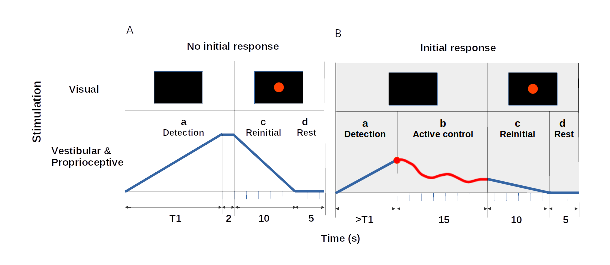
\includegraphics[width=0.9\linewidth]{figures/figure2.eps}
%\end{center}
%\caption{Experimental event timeline examples. Timeline A occurred when the participant did not respond in phase A, it consisted of three phases: (A Detection) motion stimulation of the cabin using a smoothed ramp forcing function, (C Reinitialization) cabin reinitialization to the initial orientation or position, (D Rest) cabin and participant at rest. Timeline B occurred when the participant responded in phase A, the four phases consisted of: A Detection, (B Active control) participant active control, C Reinitialization, D Rest. For both timeline A and B, visual and vestibular stimulation was given during each phase. The blue and red lines are position-based trajectories. The blue line denotes automatic robotic movement of the simulator cabin along one axis per trial, and the red line denotes the stimulus plus the participant’s movements to compensate for the perturbation. T1 denotes the maximum allowed stimulation time per trial with respect to each axis and speed, if initial detection was not made within T1s the experimental phases followed as depicted in timeline A. If the joystick was moved within T1s, an initial response was registered and experimental phases occurred as depicted in timeline B.}
%\label{fig2}
%\end{figure}
% --------------------

% --------------------
% Two figures stacked to make the figures larger and easier to see
% --------------------
\begin{figure}[htp]
\begin{center}
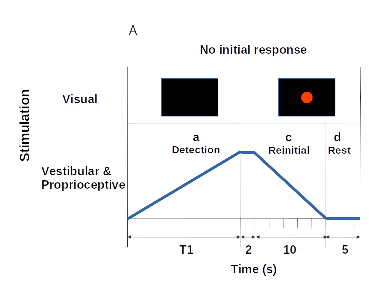
\includegraphics[width=0.9\linewidth]{figures/figure2A.eps}
\end{center}
\end{figure}

\begin{figure}[htp]
\begin{center}
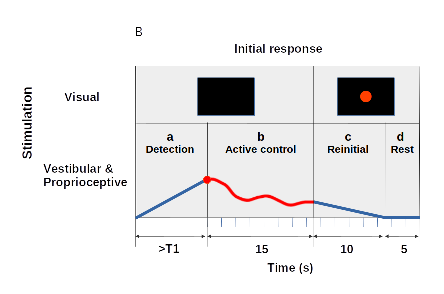
\includegraphics[width=1.0\linewidth]{figures/figure2B.eps}
\end{center}
\caption{Experimental event timelines for when participants did not respond during phase a (Timeline A) and when participants did respond (Timeline B).}
\label{fig2}
\end{figure}
% --------------------

\begin{itemize}
\item Phase a detection: A smoothed ramp-forcing function, where the rate of displacement was unknown to the participants, slowly and continuously perturbed one of the three rotational or translational axes of the simulator cabin at a sub or sup rate. The acceleration profile was the second derivative of the position trajectory. Position trajectories are shown by the blue and red lines in Figure \ref{fig2}. During phase a participants were tasked to perform ``initial detection", which consisted of identifying the axis and direction of the felt perturbation and manipulating a joystick replicating actual aircraft controls (Thrustmaster Hotas Warthog joystick), shown in Figure \ref{fig1}B, in the opposite direction of the stimulus. Participants had 15-20s to detect motion depending on the condition, denoted by T1 in Figure \ref{fig2}, which corresponded to the cabin reaching the maximum allowed cabin displacement for a particular axis and direction. T1 was different for every axis and experiment because sub and sup rates were different for each experiment and the physical cabin displacement range was different for each axis. In particular, the rotational experiment had slightly longer stimulation times than the translational experiment because the sub and sup rates were slower and the available cabin displacements in the RO, PI, and YA orientations were larger than the available translational displacement ranges. If the participants did not respond within T1s during phase A, the cabin automatically displaced along one of the three axes as the ramp function increased until it reached T1s, where the ramp function maintained a zero slope causing the cabin to remain stationary for 2s.
\item Phase b active control: If participants responded within T1s during phase A, phase B active control began and they had 15s to maintain the simulator orientation or position stably at the initial location by counteracting the perturbation; phase B was a vestibular dead-reckoning task. No visual stimulation was present; thus, the participants could rely only on vestibular and proprioceptive cues.
\item Phase c reinitialization: A red dot appeared on the screen instructing participants to release the joystick and rest, while the cabin automatically returned to the initial starting location within 10s.
\item Phase d rest: The cabin remained stationary at the starting location for 5s in order to avoid possible over-stimulation or after-effects.
\end{itemize}

\indent In summary, the shortest and longest trials were approximately 32s and 50s respectively. The shortest trial length occurred when the participant immediately responded within 1-2s (2s+15s+10s+5s) or did not respond with T1 equaling 15s ((15s+2s)+10s+5s), the longest trial length occurred when the participant responded just before T1 with T1 equaling 20s (19.9s+15s+10s+5s). Both experiments administered 42 trials: 12 familiarization practice trials and 30 experimental trials. During the familiarization practice phase, unique experimental condition combinations were given, where each of the three axes was stimulated in negative or positive directions at sub or sup speeds. Similarly, the experimental phase consisted of 30 randomized trials, in which 15 trials with unique experimental conditions were repeated twice: five direction-speed conditions (negative sup, negative sub, no-movement, positive sup, positive sub) for each of the three axes (RO/LR, PI/FB, YA/UD). No-movement trials were included as sham trials to encourage the participants to remain active.

\subsection{PARTICIPANTS}
The EuroMov Institutional Review Board (IRB) at the University of Montpellier approved that the scientific objectives and organization of both experiments (IRB-EM rotational: 1703B, IRB-EM translational: 1704B) were safe and appropriate for human participation. The EuroMov IRB committee rules and regulations are in accordance with the 1964 Declaration of Helsinki and its later amendments. Eighteen and 14 healthy volunteers with normal or corrected vision gave informed consent before participating in the rotational and translational tasks respectively (males and females, $32\pm10$ years old); four of the 32 participants reported having novice time-limited piloting experiences lasting less than 40 hours. Four of the 18 rotational and four of the 14 translational participants were over the age of 40 years. The participants who performed the rotational experiment were not the same than those who performed the translational experiment. Therefore, there was no confounds due to experimental ordering, learning, carryover, or fatigue. The same participant population, university students, and staff, was used for both experiments; therefore, it is likely that both experimental populations were similar.

\subsection{EXPERIMENTAL PROTOCOL AND MOTION SIMULATION SYSTEM}
The experiment took approximately 90 min and consisted of four sections (1) arrival, questionnaires, and instruction; (2) familiarization; (3) active control of rotational or translational stimulation; and (4) questionnaire and debriefing. After describing the experimental task and completing the questionnaires, participants were securely installed using the safety harness and communication headphones, as shown in Figure \ref{fig3}A. They were asked to moderately move the joystick in one axis direction at a time while compensating the unknown perturbation. Participants were reminded to maintain the cabin at the initial trial position or orientation, fixed at a steady centered pose, by compensating the motion stimulus. Participants were free to adopt their own strategy to perform the task, both in terms of response speed and of exploration behavior. In order to replicate a realistic flight scenario, the participants were free to move their head and body, looking and/or fixating where they wished, as long as it did not interfere with the task. The fact that the head was left unrestrained is considered undesirable, causing erroneous motion detection due to conflicting self-generated sensory information, and thus rarely performed in traditional motion perception experiments. However we considered it ecologically innovative because it replicated human response under realistic flight circumstances, allowing for a more realistic SD dataset. Once the participant was installed in the cabin, the cabin door was closed and all communication between the participant and experimenter was performed via a camera interface system that facilitated two-way auditory communication. The camera system also provided the experimenter visual feedback of the participant's upper body. The experimenter visually monitored the well-being of the participants, and confirmed participant's feelings of illness auditorily; the experiment ended if the participants reported physical illness.

% -------------------- Figure 3 --------------------
\begin{figure*}[htp]
\begin{center}

\includegraphics[width=1.0\linewidth]{figures/figure3.eps}
\end{center}
\caption{Motion simulator apparatus and installation; A and B show the experimental simulator cabin with and without a seated participant respectively. C shows an exterior view of the six-axis iMose motion simulator, consisting of the participant cabin and the robotic arm.}
\label{fig3}
\end{figure*}
% --------------------

\indent The motion simulation system that provided sensory stimulation, iMose, consisted of a 6DOF position-controlled KUKA-based motion simulator system (KR 500-3 MT adapted by BEC GmbH motion simulators, KUKA Roboter GmbH, Germany) and a local area network of three 1independent workstations \cite{Denquin_2021_LAF}, \cite{Landrieu_2017_Timetocollision}, \cite{Bellmann_2011_DLR}. Figures \ref{fig3}B and 3\ref{fig3}C show the interior and exterior of the simulation system, data was transferred between the simulator and workstations at 250 Hz on a private network using UDP. Workstations 1 and 3 were located in the experimenter control room; workstation 1 generated motion for the robot using a MATLAB/Simulink control interface program (MATLAB and Simulink Toolbox Release 2009, The MathWorks, Inc., Natick, Massachusetts, USA). Workstation 2 was fixed to the simulator cabin, and it administered the red dot or black visual screen and recorded the streamed user-controlled joystick signal. Workstation 3, using Labview, served as the experimenter’s user control interface to start and stop the experiment and collect experimental data without causing information delays between the workstations.

\indent Two questionnaires were administered before the experimental phase: a claustrophobia assessment \cite{Radomsky_2001_Claustrophobia}, \cite{Radomsky_2006_Claustrophobia_CLQ} and SSQ \cite{Kennedy_1993_Simulator}, \cite{Bouchard_2007_SimulatorSickness}. All questionnaires were administered in the native fluently spoken language of each participant (French or English). The claustrophobia questionnaire consisted of two sections: the first section measured fear of suffocation (14 questions) and the second section assessed fear of restriction (12 questions). The claustrophobia questionnaire was used as a screening method to assess whether participants could enter the simulator and perform the task relatively stress-free; participants who scored 40 points or lower, indicating that they were not claustrophobic, were initially recruited, and participants scoring higher than 40 were recruited last. For both the rotational and translational experiments all participants scored “non-claustrophobic”, rotational results were mean=10.94, max=38, min=0 and translational results were mean=8.77, max=9, min=0. The SSQ consisted of 16 questions and measured the participant’s general physical state, evaluating nausea, ocular motor, and disorientation sub-scales. The SSQ was administered before and after the experiment to measure the effects of the experiment in terms of disorientation.
